\chapter{Resultados e Discussão}\label{cap:resultados}

Após entender o funcionamento do algoritmo de Viola Jones, foram executados testes com os conjuntos de imagens selecionados e os resultados obtidos são discutidos a seguir.

Inicialmente, foi necessário especificar com clareza como poderiam ser agrupadas as imagens, dada a sua origem e o resultado observado no teste, para isso foram utilizadas as definições da tabela \ref{tab:grupos-images}. 

\begin{table}[htbp]
    \caption{Grupos observados}
    \label{tab:grupos-images}
    \centering
    \begin{tabular}{ccc}\hline\hline
        \textbf{Grupo} & \textbf{Descrição} & \textbf{Quantidade} \\\hline
        \textit{A} & Imagens que não contêm nenhuma face & 17130 \\
        $\overline{A}$ & Imagens que contêm uma face & 17130 \\
        \textit{B} & Imagens onde o algoritmo não identificou nenhuma face & Variável \\
        $\overline{B}$ & Imagens onde o algoritmo identificou uma ou mais faces & Variável \\
    \hline\hline
    \end{tabular}
\end{table}

Definidos os grupos, pode-se utilizar a tabela de contingência \ref{tab:tabela_contingencia} para facilitar a análise da relação entre os grupos definidos anteriormente. Na tabela \ref{tab:tabela_contingencia} são observados os grupos \textit{a} (verdadeiro positivo) onde o algoritmo identifica corretamente uma face em cada uma das imagens que realmente contêm uma face, \textit{b} (falso negativo) onde o algoritmo erroneamente não reconheceu nenhuma face, apesar das imageens conterem uma face cada, \textit{c} (falso positivo) onde o algoritmo erroneamente identificou ao menos uma face, mesmo as imagens não contendo nenhuma e \textit{d} (verdadeiro negativo) onde o algoritmo identificou corretamente que não existia nenhuma face nas imagens. É importante destacar que os quatro grupos destacados na tabela de contingência são mutuamente excludentes. \cite{Dougherty:2012:PRC:2553126}

\begin{table}[htbp]
    \caption{Tabela de contingência}
    \label{tab:tabela_contingencia}
    \centering
    \begin{tabular}{ccc}\hline\hline
        & \textit{B} & $\overline{B}$ \\
    \textit{A} & \textit{a} (verdadeiro positivo) & \textit{b} (falso negativo) \\
    $\overline{A}$ & \textit{c} (falso positivo) & \textit{d} (verdadeiro negativo) \\
    \hline\hline
    \end{tabular}
\end{table}

Para melhor entender os agrupamentos da tabela de contingência, pode-se observar na imagem \ref{fig:norm_dist} as distribuições que representam a quantidade de imagens dos grupos \textit{A} e $\overline{A}$ dada a sua probabilidade de conter uma face. 

\begin{figure}[htbp]
    \centering
    \caption{Possível distribuição normal dos grupos observados na tabela de contingência.}
    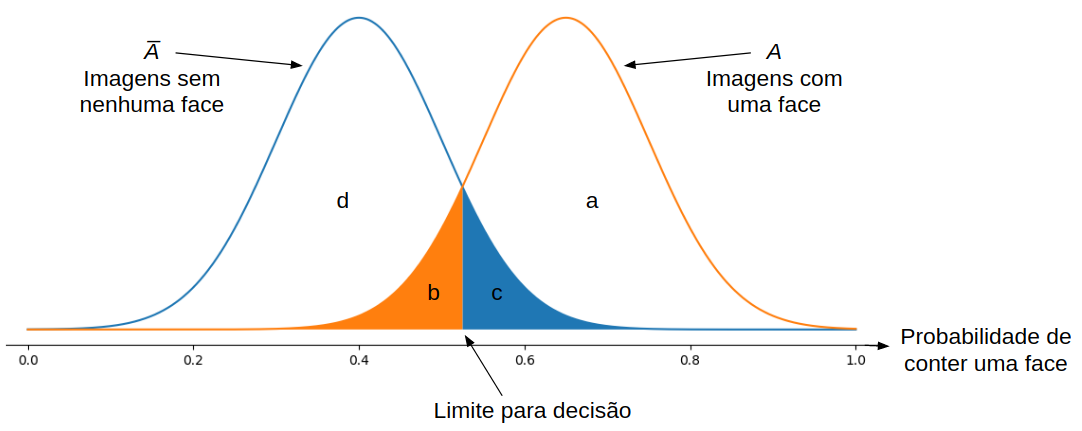
\includegraphics[scale=.5]{figs/norm_dist.png}
    \label{fig:norm_dist}
 \end{figure}

 Nas distribuições são destacados os grupos \textit{b} (falso negativo) e \textit{c} (falso positivo) e fica evidente que, devido a sobreposição das distribuições \textit{A} e $\overline{A}$, é necessário definir uma limite para decisão, que pode ser ajustado conforme a necessidade, mas que independente do seu ajuste, sempre existirá um grupo categorizado de forma incorreta.

 A tabela de contingência também pode ser escrita em termos probabilísticos (tabela \ref{tab:tabela_contingencia_probab}), incluindo as probabilidades marginais ou pode ser visualizada no diagrama de Venn correspondente (figura \ref{fig:venn_diagram}).

\begin{table}[htbp]
    \caption{Tabela de contingência com probabilidades marginais}
    \label{tab:tabela_contingencia_probab}
    \centering
    \begin{tabular}{cccc}\hline\hline
        & \textit{B} & $\overline{B}$ & Soma\\
    \textit{A} & $P(A \cap B)$ & $P(A \cap \overline{B})$ & $P(A)$ \\
    $\overline{A}$ & $P(\overline{A} \cap B)$ & $P(\overline{A} \cap \overline{B})$ & $P(\overline{A})$ \\
    Soma & $P(B)$ & $P(\overline{B})$ & 1 \\
    \hline\hline
    \end{tabular}
\end{table}

 \begin{figure}[htbp]
     \centering
     \caption{Diagrama de Venn para as imagens analisadas.}
     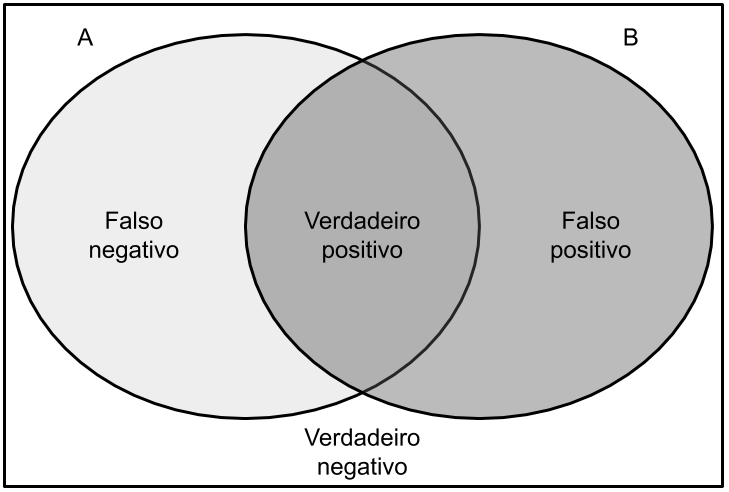
\includegraphics[scale=.4]{figs/venn-diagram.png}
     \label{fig:venn_diagram}
  \end{figure}

Por fim, podem ser calculadas as medidas tradicionais de sensitividade (a probabilidade condicional do algoritmo identificar ao menos uma face dado que a imagem contém uma face) e especificidade (a probabilidade condicional do algoritmo não identificar nenhuma face em uma imagem que realmente não contém nenhuma face) conforme as equações \ref{eq:sensitividade} e \ref{eq:especificidade}.

\begin{align} \label{eq:sensitividade}
    \text{sensitividade, } P(B|A) = P(A \cap B) / (P(A \cap B) + P(A \cap \overline{B})) = a/(a + b) \\
    \label{eq:especificidade}
    \text{especificidade, } P(\overline{B} | \overline{A}) = P(\overline{A} \cap \overline{B}) / (P(\overline{A} \cap \overline{B}) + P(\overline{A} \cap B)) = d/(d + c)
\end{align}

A biblioteca OpenCV permite ainda ajuste de parâmetros para a execução do algoritmo de Viola Jones, neste teste, serão utilizados: o fator de escala, que é o fator pelo qual as dimensões da imagem serão multiplicadas na tentativa de encontrar faces de diferentes tamanhos (quanto menor, maior a chance de encontrar faces) e o número mínimo de vizinhos, que é número mínimo de detecções, após varias iterações, para uma parte da imagem ser considerada uma face (quanto menor, maior a chance de encontrar faces).

Na primeira iteração executada sobre o conjunto de imagens, foram ajustados os parâmetros de fator de escala para 1.3 e número mínimo de vizinhos para 5, após analisar todas imagens foi possível preencher a tabela de contingência \ref{tab:tabela_contingencia_teste1} e calcular a respectiva sensitividade $P(B|A) = 98.5872\%$ e especificidade $P(\overline{B} | \overline{A}) = 86.6024\%$.

\begin{table}[htbp]
    \caption{Tabela de contingência com os resultados do primeiro teste}
    \label{tab:tabela_contingencia_teste1}
    \centering
    \begin{tabular}{cccc}\hline\hline
        & \textit{B} & $\overline{B}$ & Soma\\
    \textit{A} & 49.2936\% & 00.7064\% & 50\% \\
    $\overline{A}$ & 06.6988\% & 43.3012\% & 50\% \\
    Soma & 55.9924\% & 44.0076\% & 100\% \\
    \hline\hline
    \end{tabular}
\end{table}

Na segunda iteração, ajustando o fator de escala para 1.05 e o número mínimo de vizinhos para 3, foram obtidos os resultados apresentados na tabela \ref{tab:tabela_contingencia_teste2} e a respectiva sensitividade $P(B|A) = 66.3923\%$ e especificidade $P(\overline{B} | \overline{A}) = 98.3479\%$.

\begin{table}[htbp]
    \caption{Tabela de contingência com os resultados do segundo teste}
    \label{tab:tabela_contingencia_teste2}
    \centering
    \begin{tabular}{cccc}\hline\hline
        & \textit{B} & $\overline{B}$ & Soma\\
    \textit{A}& 33.1962\% & 16.8038\% & 50\% \\
    $\overline{A}$& 00.8260\% & 49.1740\% & 50\% \\
    Soma& 34.0222\% & 65.9778\% & 100\% \\
    \hline\hline
    \end{tabular}
\end{table}

Observando as duas iterações, o primeiro ponto de destaque é o impacto dos parâmetros nos resultados, comparando as medidas de \textit{B} na primeira e segunda iterações, percebe-se que a redução dos valores ajustados tanto nos parâmetros de fator de escala e número de vizinhos, fez com que mais faces forem detectadas, conforme o esperado, consequentemente, ouve um grande aumento no número de falsos negativos, onde o algoritmo encontra uma face apesar da mesma não existir. 

Analisando a sensitividade, percebe-se que na segunda iteração essa foi bastante reduzida, ou seja, dado o grupo de imagens que não possuíam nenhuma face, na primeira iteração 98.5872\% delas foram classificadas corretamente como imagens sem nenhuma face, já na segunda iteração somente 66.3923\% foram classificadas corretamente.

Já analisando a especificidade, o valor teve uma redução na segunda iteração, mas não foi uma variação tão significativa quanto a variação da sensitividade, este dado pode ser entendido da seguinte forma, dado o grupo de imagens que possuíam uma face, na primeira iteração 86.6024\% delas foram classificadas corretamente como imagens com ao menos uma face e na segunda iteração 98.3479\% foram classificadas corretamente.

Vale enfatizar que ambas análises sensitividade e especificidade estão de acordo com os resultados esperados devido aos parâmetros utilizados que fazem com que a segunda iteração detecte uma quantidade maior de faces.

Outro ponto a ser destacado é a porcentagem de imagens classificadas corretamente, ou seja, a soma das porcentagens de verdadeiros positivos e verdadeiros negativos, que na primeira iteração foi igual a 92.5948\% e na segunda iteração foi igual a 82.3702\%, esses valores demonstram que a ajuste de parâmetros não influencia apenas no limite de decisão observado na figura \ref{fig:norm_dist}, mas também nas distribuições.

Relembrando o objetivo do projeto, que consiste em negar rapidamente imagens que certamente não possuem nenhuma face, e observando os resultados obtidos e análisados, pode-se concluir que o algoritmo de Viola Jones implementado na biblioteca OpenCV poderia ser utilizado de forma satisfatória para solucionar tal problema. Além disso, a utilização dos parâmetros ajustados na primeira iteração se mostra mais adequada, devido a maior quantidade de imagens classificadas corretamente, que torna possível negar de forma correta e automática 98.5872\% das imagens que não possuem faces, mas é importante lembrar que 13.3976\% das imagens que possuem uma face seriam também automáticamente negadas erroneamente. Para os casos onde negar uma imagem correta poderia causar maiores problemas, é recomendável utilizar os mesmos parâmetros da segunda iteração, que tornaria possível negar de forma correta e automática 66.3923\% das imagens que não possuem faces, mantendo em apenas 1.6521\% o volume de imagens que possuem uma face seriam  automáticamente negadas erroneamente.